\section{Etude sur MNIST}
\subsection{Comparaison de deux réseaux en fonction du pré-apprentissage} 

Dans cette section, nous allons évaluer les performances du Deep Neural Network sur le jeu de données MNIST en fonction de l'entraînement préalable du réseau. Nous allons examiner les performances pour différentes valeurs de paramètres, tels que le nombre de couches du réseau, le nombre de neurones par couche et la quantité de données d'entraînement utilisées. Pour toutes les comparaisons, nous avons utilisé un nombre fixe d'itérations pour les descentes de gradient, à savoir 100 pour les RBM et 200 pour l'algorithme de rétropropagation du gradient. De plus, nous avons utilisé un taux d'apprentissage de 0,1 et une taille de mini-batch de 64.


\subsection{Comparaison selon le nombre de couches}

\begin{figure}[H]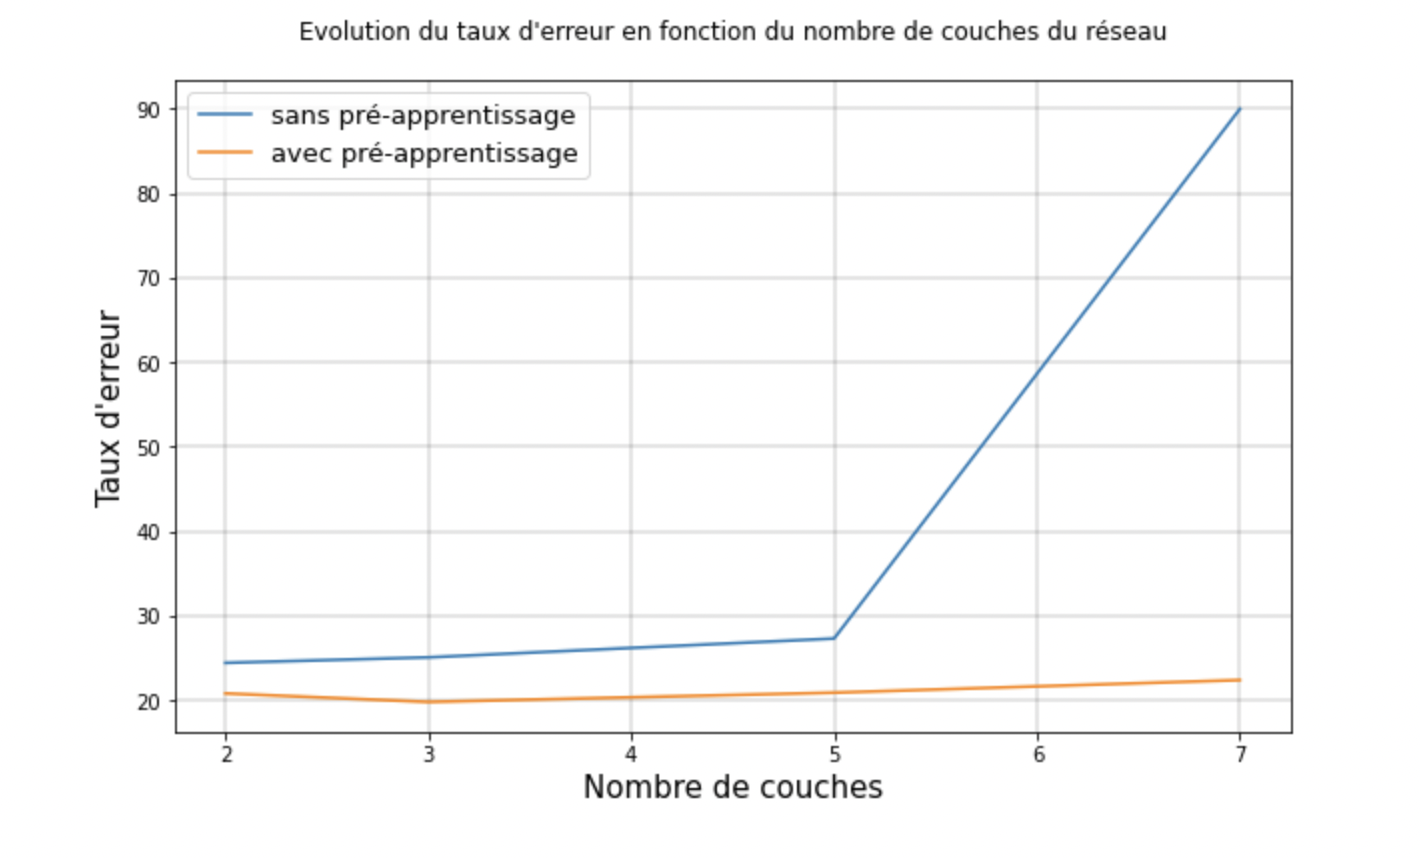
\includegraphics[width=140mm]{images/DNN1.png}
\caption{Variation du taux d'erreur en fonction du nombre de couches dans un DNN}
\end{figure}
En examinant la Figure 3, on constate que le nombre de couches n'a pas un impact significatif sur la précision, comme le montre le taux d'erreur (1-précision). Cependant, pour les réseaux sans entraînement préalable, on observe une forte augmentation du taux d'erreur à partir de 5 couches. Ces résultats ont été obtenus en utilisant 60000 données et un nombre de neurones par couche de 200.


\subsection{Comparaison selon le nombre de neurones par couches}

\begin{figure}[H]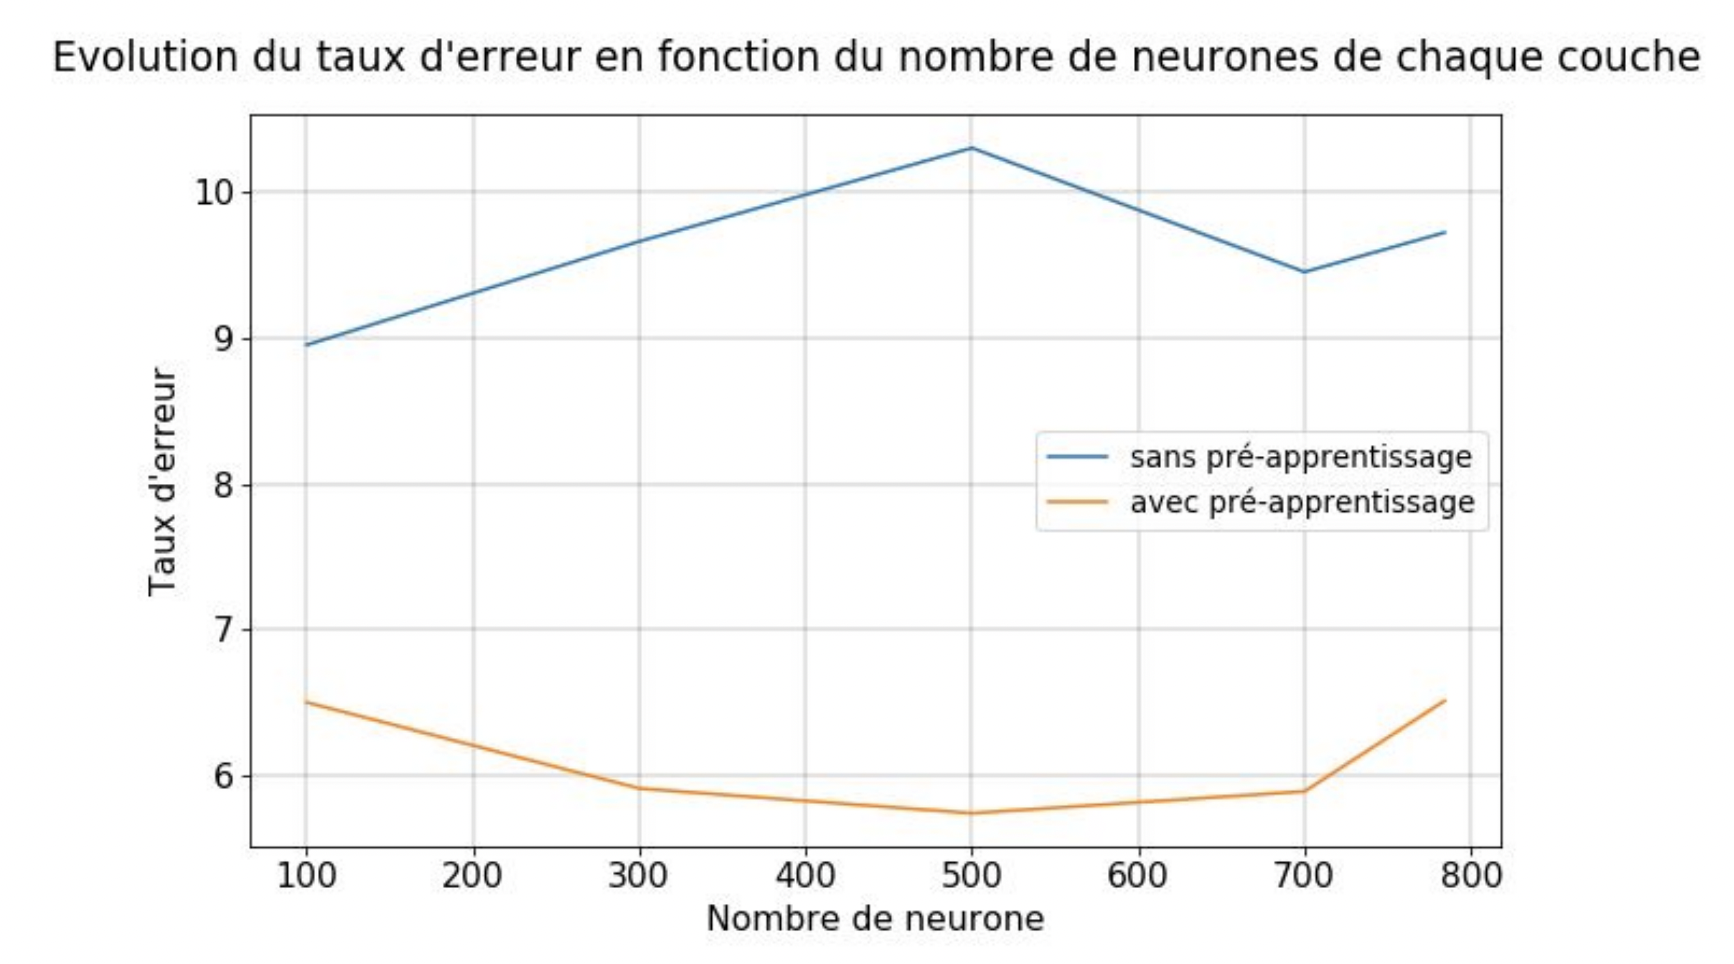
\includegraphics[width=140mm]
{images/graph1.png}
\caption{Taux d'erreur en fonction du nombre de neurones par couche}
\end{figure}
La Figure 4 révèle que la précision du réseau pré-entraîné augmente à mesure que le nombre de neurones par couche augmente. Cependant, pour le réseau non-entraîné, on observe une augmentation de l'erreur lorsque le nombre de neurones par couche est augmenté. Ces tests ont été réalisés en utilisant 2 couches et 60000 données.

\subsection{Comparaison selon le nombre de neurones par couches}

\begin{figure}[H]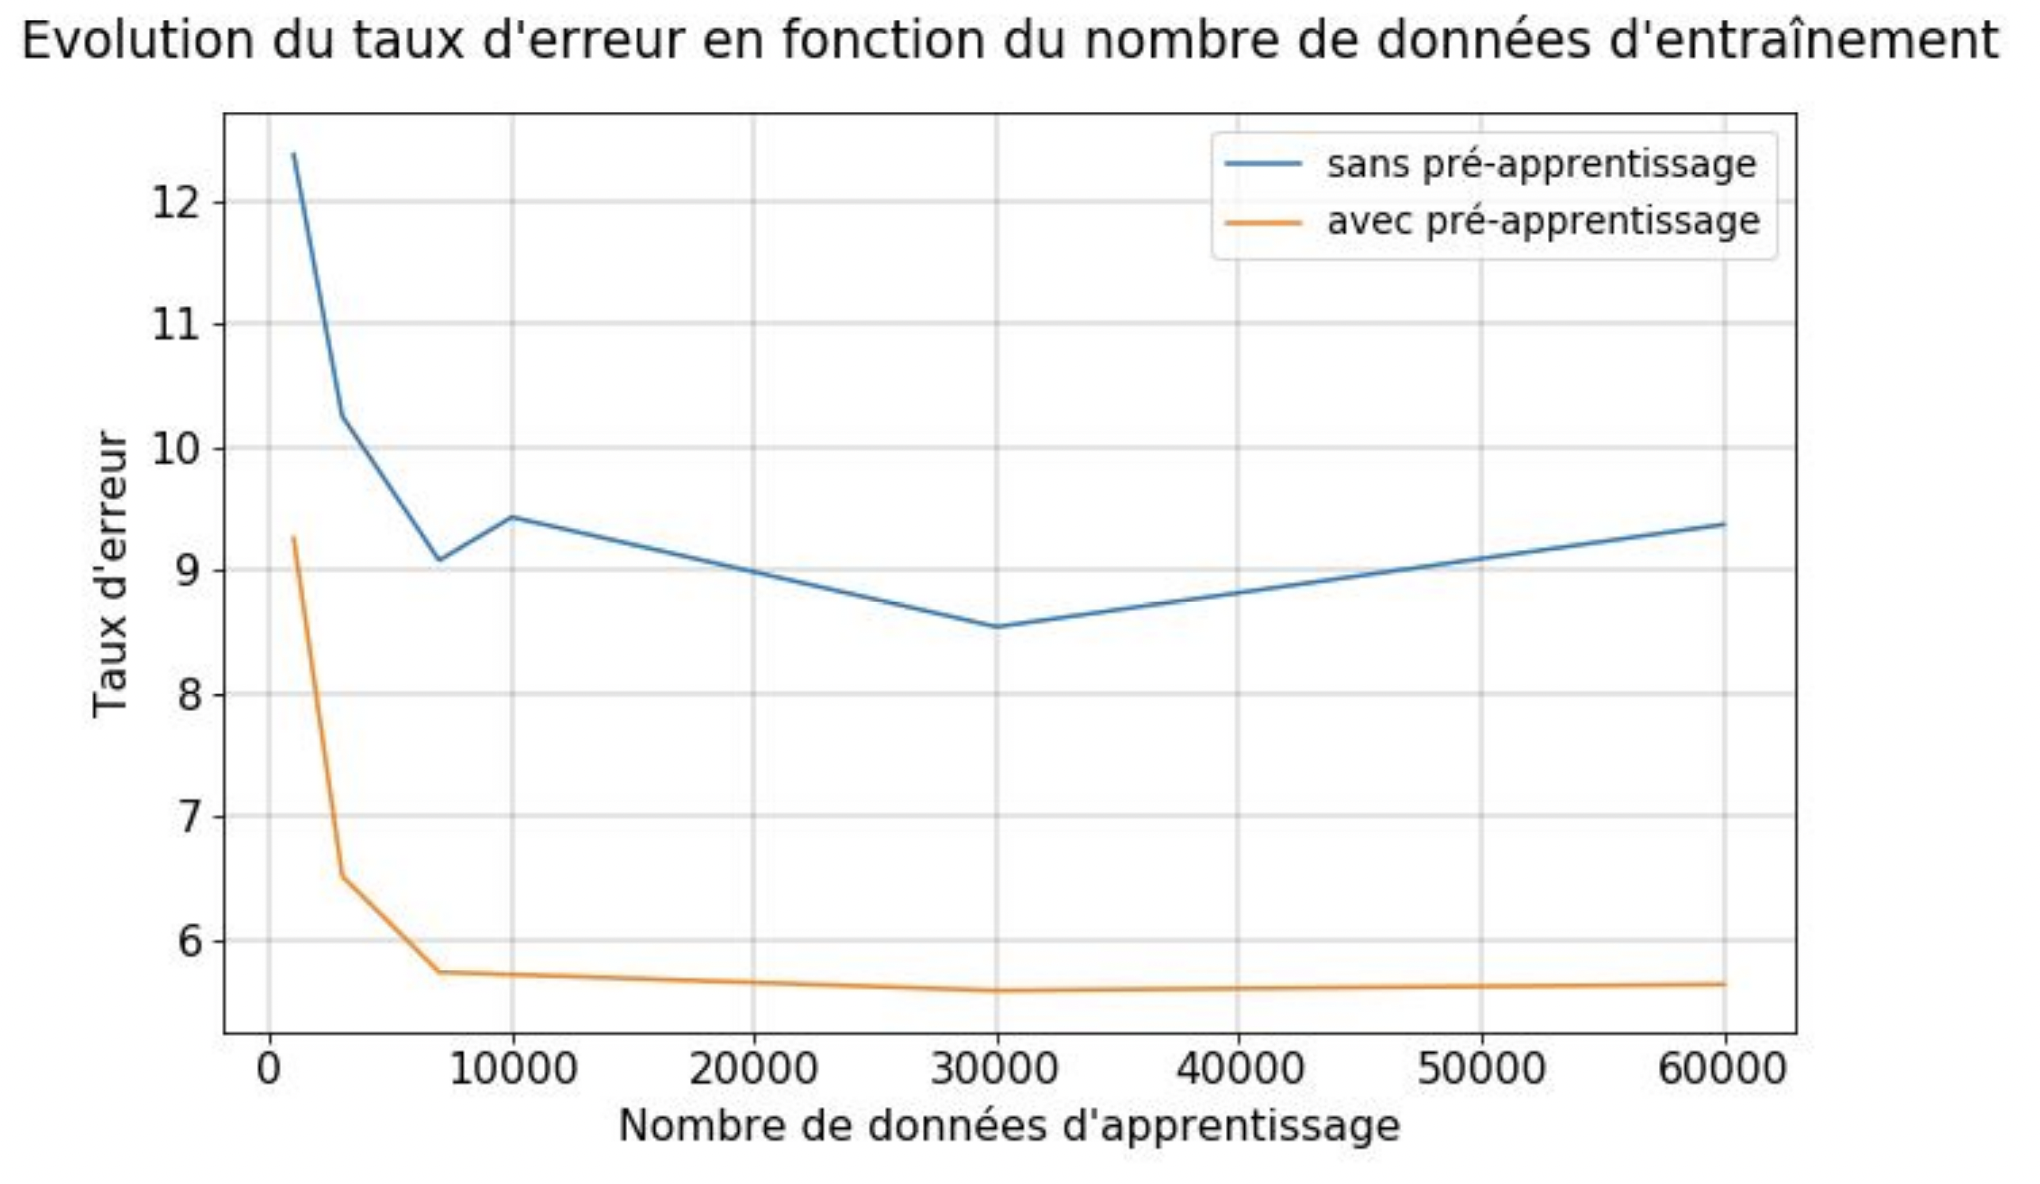
\includegraphics[width=140mm]
{images/graph2.png}
\caption{Variation du taux d'erreur en fonction de la quantité de données pour des DNN entraînés avec ou sans pré-apprentissage.}
\end{figure}
La Figure 5 indique que pour les deux réseaux, la précision augmente et l'erreur diminue à mesure que le nombre de données d'entraînement augmente. Cependant, on remarque également un taux d'erreur minimum lorsqu'on entraîne le réseau avec 30 000 données. Ces tests ont été réalisés en utilisant 2 couches et 200 neurones par couche.\\
En analysant ces trois comparaisons, on constate que le réseau pré-entraîné présente un taux d'erreur nettement inférieur à celui du réseau non-entraîné. Cependant, il convient de noter que le temps de calcul requis pour le pré-apprentissage est très élevé.

\subsection{Comparaison selon le learning rate}

La Figure 6 permet de déterminer le learning rate optimal pour un réseau entraîné avec 60 000 données, qui est de 0,425 dans notre cas. De manière générale, plus le LR est élevé, plus le taux d'erreur est bas. Cependant, la valeur de 0,425 permet une nette amélioration du taux d'erreur pour notre problème.

\begin{figure}[H]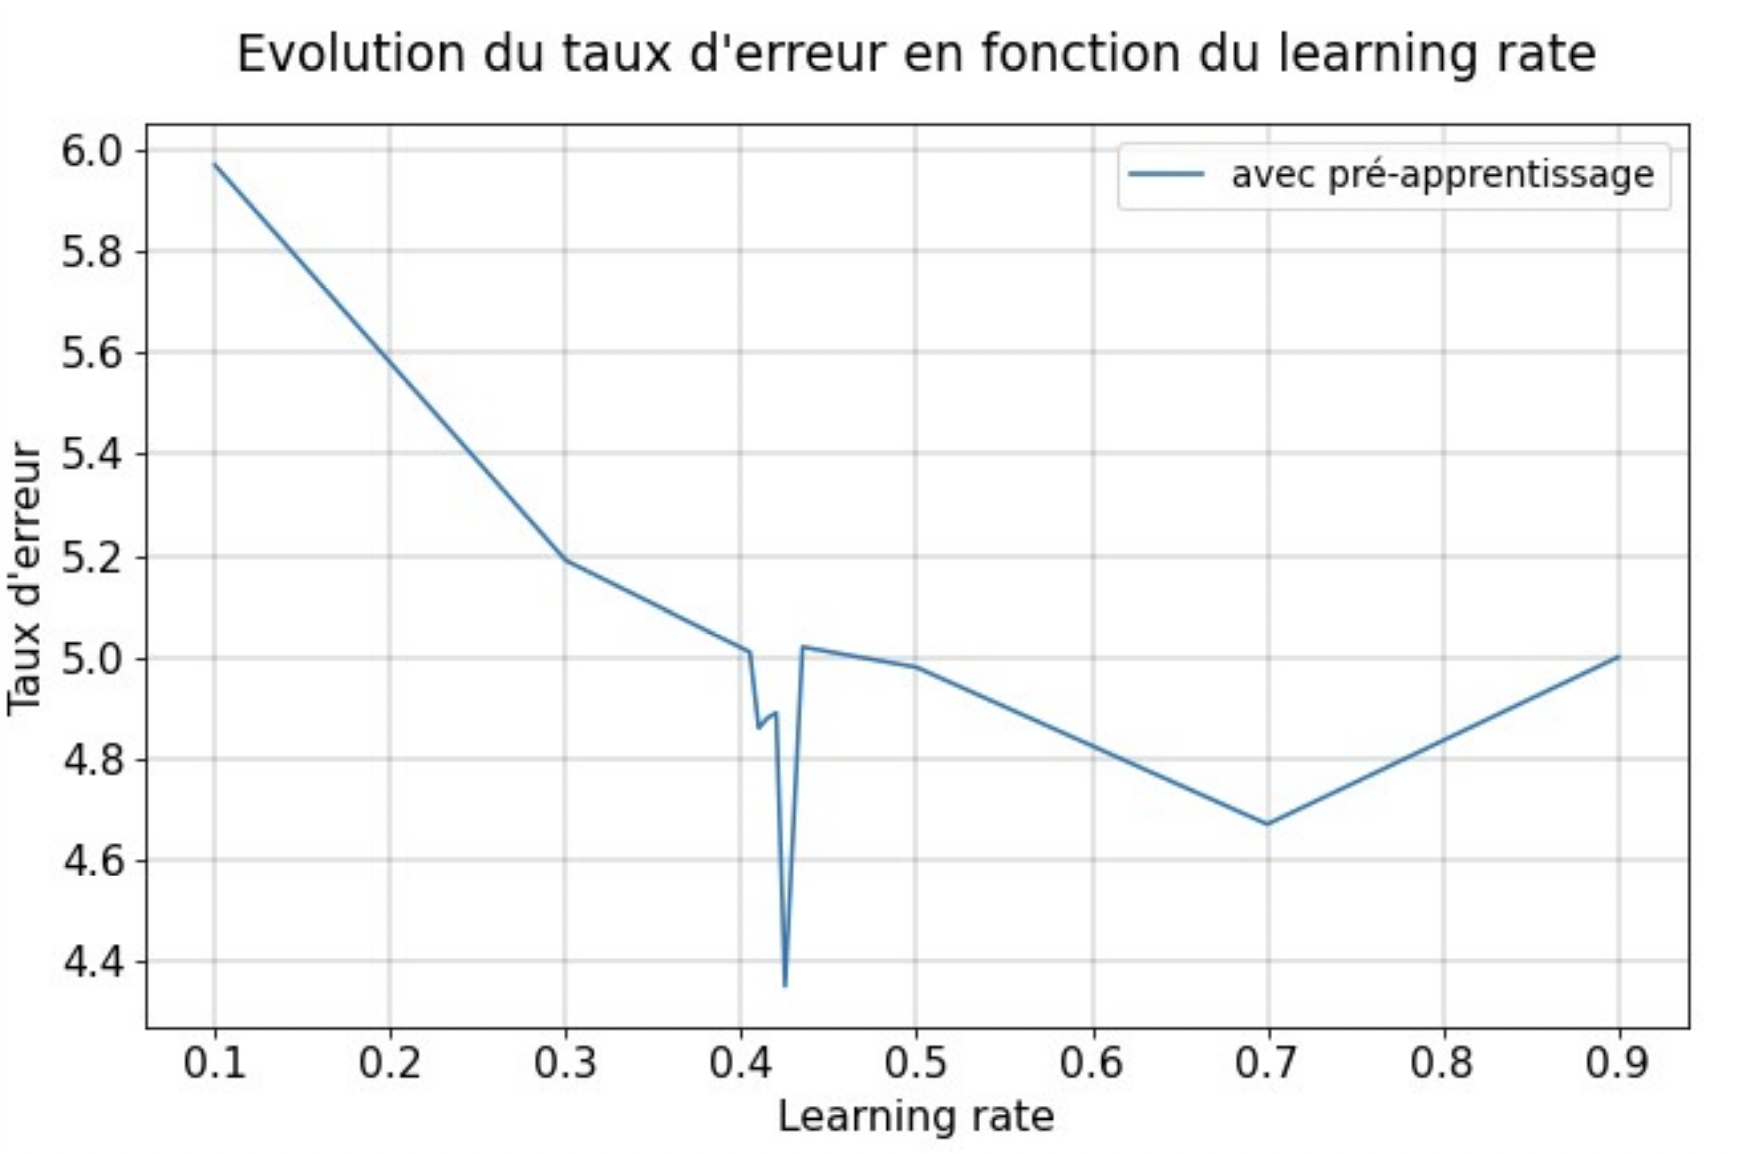
\includegraphics[width=140mm]
{images/graph3.png}
\caption{Variation du taux d'erreur en fonction du learning rate.}
\end{figure}

\subsection{Meilleur taux de classification}
En se basant sur les comparaisons précédentes, nous avons cherché à déterminer les paramètres optimaux pour obtenir le taux d'erreur le plus faible possible sur les données de test. Nous avons ainsi obtenu un taux d'erreur de 2,74\% en utilisant les paramètres présentés dans le tableau ci-dessous :


\begin{table}[h!]
\centering
\begin{tabular}{|c|c|}
\hline
Paramètre & Valeur \\
\hline
Nombre d’itérations (RBM)  & 100 \\
Nombre d’itérations (Rétro-Propagation) & 350  \\
Taille des mini-batch & 128 \\
Learning Rate & 0.425  \\
Nombre de données d’apprentissage & 30 000  \\
Nombre de couches & 4  \\
Nombre de neurones par couche & 200  \\
\hline
\end{tabular}
\end{table}
